\documentclass{article}

\usepackage{amsmath, amssymb}
\usepackage{tikz, color, ifthen}
\usepackage{geometry}[fullpage]
\usetikzlibrary{calc}

\newcommand{\cellwidth}{28}

\newcommand{\drawEnergyLine}[2]{
  %% Draws a diagram highlighting energy lines required for monte carlo
  %% Arguments:
  %%     #1: x-pos of targeted cell
  %%     #2: y-pos of targeted cell
  \foreach \i in {1, ..., 9} {
    \foreach \j in {1, ..., 9} {
      \ifthenelse{\i = #1 \OR \j = #2}{
        \ifthenelse{\i = #1 \AND \j = #2}{
          \node at (\i, -\j) {\underline\i\underline\j};
        }{
          \ifthenelse{\j = #2} {
            \node at (\i, -\j) {\i\underline\j};
          }{
            \node at (\i, -\j) {\underline\i\j};
          }
        }
      }{
        \node[cell] at (\i, -\j) {\i\j};
      }
    };
  };
}

\newcommand{\drawEnergyLineTwo}[2]{
  %% Draws a diagram highlighting energy lines required for monte carlo
  %% Arguments:
  %%     #1: x-pos of targeted cell
  %%     #2: y-pos of targeted cell
  \foreach \i in {1, ..., 9} {
    \foreach \j in {1, ..., 9} {
      \ifthenelse{\i = #1 \OR \j = #2}{
        \ifthenelse{\i = #1 \AND \j = #2}{
          \node at (\i, -\j) {\underline\i\underline\j};
        }{
          \ifthenelse{\j = #2} {
            \node at (\i, -\j) {\i\underline\j};
          }{
            \node at (\i, -\j) {\underline\i\j};
          }
        }
      }{
        \node[cell] at (\i, -\j) {\i\j};
      }
    };
  };
}


\newcommand{\multiCell}[2]{
  %% Draws a cell with optional diagonal slash denoting two different colours.
  %%
  %% Arguments
  %%     #1 int
  %%         x-position of cell
  %%     #2 int
  %%         y-position of cell
  %%     #3 colou
  %%         north west corner colour
  %%     #4 colou
  %%         south east corner colour
  \node [cell, name=multiCell] at (#1, #2) {};

  % north east corner colour
  \filldraw[green!80] (multiCell.south west)
  -- (multiCell.north west)
  -- (multiCell.north east)
  -- cycle;

  % south east corner colour
  \filldraw[yellow!80] (multiCell.south west)
  -- (multiCell.south east)
  -- (multiCell.north east)
  -- cycle;
}


\begin{document}

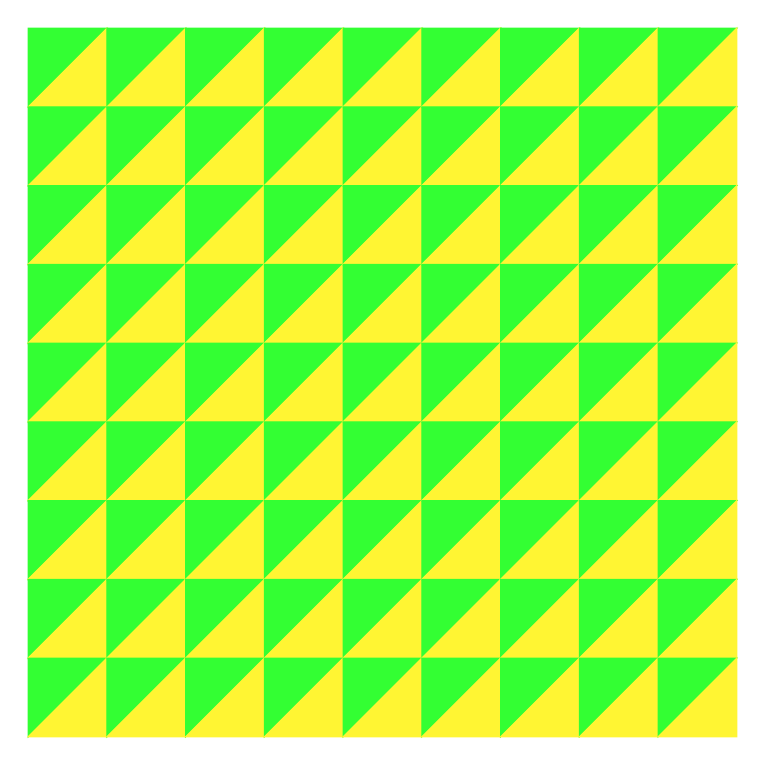
\begin{tikzpicture}
  [
    cell/.style={
      rectangle,
      draw,
      minimum width=\cellwidth,
      minimum height=\cellwidth,
    }
  ]
  \foreach \i in {1, ..., 9} {
    \foreach \j in {1, ..., 9} {
      \multiCell{\i}{-\j}
    }
  }

\end{tikzpicture}

\newpage

\section*{Sudoku}
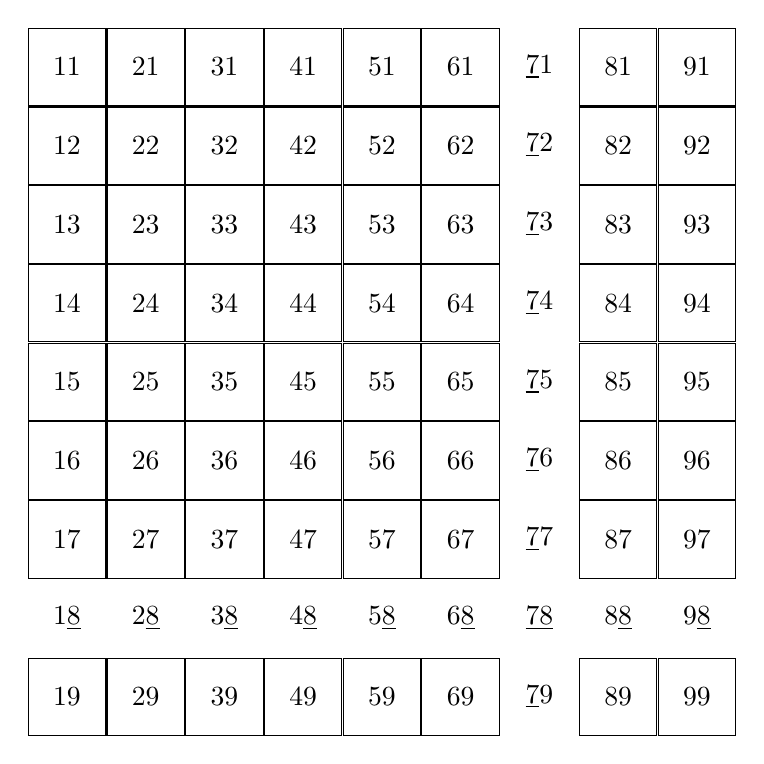
\begin{tikzpicture}[
    cell/.style={
      rectangle,
      draw=black,
      minimum width=\cellwidth,
      minimum height=\cellwidth
    }
  ]
  \drawEnergyLine{7}{8}
\end{tikzpicture}

\newpage

\section*{Double Sudoku}
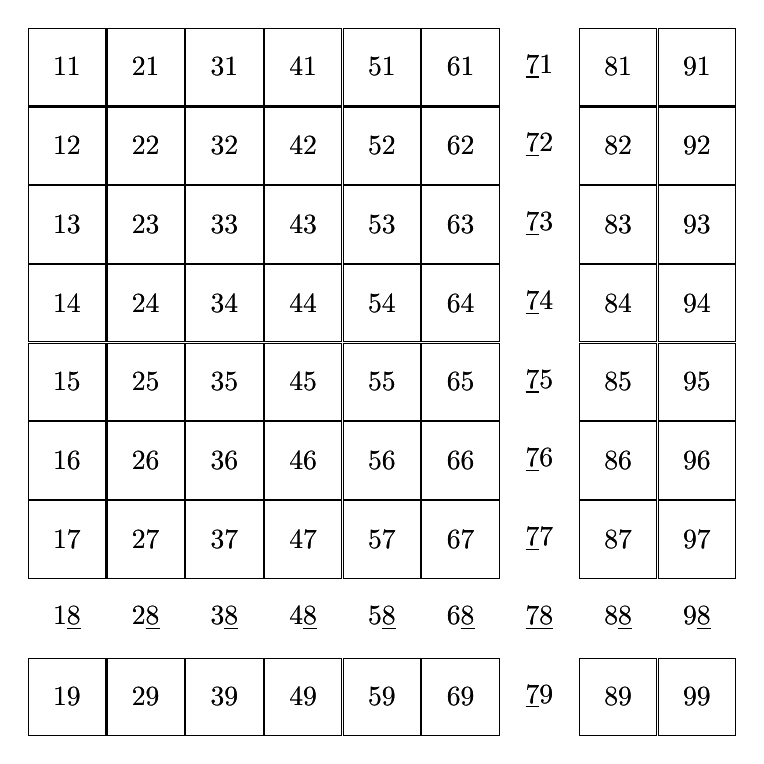
\begin{tikzpicture}[
    cell/.style={
      rectangle,
      draw=black,
      minimum width=\cellwidth,
      minimum height=\cellwidth
    }
  ]
  \drawEnergyLine{7}{8}
  \drawEnergyLineTwo{7}{8}
\end{tikzpicture}
\end{document}
